\section{09. Mai 2012}

\question{Skizzieren der wesentlichen Elemente der Born-Oppenheimer Näherung.}
\label{q:21}

Da die Atomkerne eine wesentlich größere Masse als die Elektronen haben und sich dadurch viel langsamer bewegen, ist es mit der Born-Oppenheimer
Näherung möglich die Positionen der Kerne zu fixieren. Somit lässt sich die molekulare Schrödingergleichung in eine für die Kerne und eine
für die Elektronen aufteilen.

\begin{itemize}
    \item Für die Elektronen stehen die Kerne still, wodurch ihre Lage als Parameter in das anziehende und abstoßende Potential eingeht.
        Somit hängen die elektronischen Eigenzustände und Energien nur von der Lage der Kerne ab und nicht von der Geschwindigkeit.\\
            Die Schrödingergleichung für die Elektronen lautet somit:
            
        \begin{align}
            \hat{H}_e * \Phi_h(\vec{r},\vec{R}) = E_h(\vec{R}) *  \Phi_h(\vec{r},\vec{R})
        \end{align}

        Dabei ist $\vec{r}$ die Position der Elektronen und $\vec{R}$ die der Kerne. Der Hamiton besteht aus $\hat{H}_e = \hat{T}_e + \hat{V}_{ee} + \hat{V}_{eN}$, 
        also der kinetischen Energie der Elektronen + der Abstoßung zwischen den Elektronen + der Anziehung zwischen Kernen und Elektronen.

        \begin{figure}[H]
            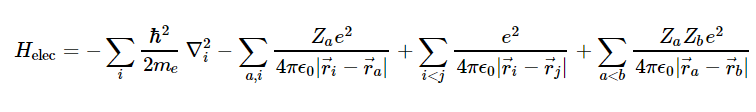
\includegraphics[width=0.8\linewidth]{resources/09-05-2012/born_op.PNG}
            \caption{Elektronischer Hamiton}
        \end{figure}

    \item Die Kernbewegeung ist von den Elektronen nahezu unbeeinflusst, jedoch bewegen sie sich im Potential der elektrischen Zustände. 
        Die Kern-Wellenfunktion $\eta_{hk}(\vec{R})$ hängt nur von der Kernkoordinate $\vec{R}$ ab.\\
        Die Schrödingergleichung lautet: 

        \begin{align}
            (\hat{T}_n + \hat{V}_{NN} + E_h(\vec{R})) * \eta_{hk}(\vec{R}) = E_{hk} * \eta_{hk}(\vec{R})
        \end{align}
\end{itemize}



\question{Welche Informationen über molekulare Kerngrößen können aus Rotations-Schwingungsspektren von Molekülen erhalten werden?}
\label{q:22}
\begin{itemize}
    \item Rotationskonstanten $B_e$ und $\alpha_e$ 
    \item Gleichgewichtsabstand $R_e$
    \item Form der Potentialkurve
\end{itemize}
Die Rotationsenergieniveaus eines Moleküls sind direkt mit dessen Massenverteilung verbunden.
Die Kenntniss der Emissionslinien bzw. Absorbtionlinien (meistens > 800 nm) ermöglicht es das Trägheitsmoment $I$ des Moleküls zu bestimmen. 
\begin{align}
    E_{rot} &= \frac{\vec{J}^2}{2 I } \\
    E_{rot} &= \frac{J(J+1)\hbar^2}{2I} \hspace{0.5cm} J = 0,1,2 \hspace{0.5cm} \text{QM}\\
    \Delta E_[rot] &= \frac{(J+1)\hbar^2}{I}
\end{align}
Meist wird die Energie in der Spektroskopie in Form von Wellenzahlen (m$^{-1}$) angegeben, dies entspricht der räumlichen Frequenz der emettierten bzw absorbierten E-Welle.
So kann ein Zusammenhang zur Rotationskonstante $B_e$ hergestellt werden.
\begin{align}
    F_{rot}(J) &= \frac{E_{rot}(J)}{h c} = B_e J(J+1) \\
    B_e &= \frac{\hbar}{4 \pi c I}
\end{align}
\question{Diskutieren das Schwigungs-Rotations Spektrum eines 2-atomigen Moleküls.}
\label{q:23}

\question{Welche Verbesserungen des einfachen MO- oder VB-Ansatzes ermöglichen eine bessere Übereinstimmung mit den experimentellen Werten?}
\label{q:24}
\textbf{Elektroneninteraktion}:\\
Ein Ansatz zur Verbesserung des MO- oder VB-Ansatzes besteht darin, die Elektronenkorrelation zu berücksichtigen. 
Der einfache Ansatz vernachlässigt die Wechselwirkungen zwischen Elektronen, was zu Fehlern bei der Berechnung der Bindungsenergien und der Geometrie führen kann. 
Die Elektronenkorrelation kann durch Methoden wie der Konfigurationswechselwirkung (CI) oder der Dichtefunktionaltheorie (DFT) berücksichtigt werden. 
Diese Methoden erlauben eine bessere Behandlung der Elektronenkorrelation und führen zu genaueren Ergebnissen.
\textbf{Relativistische Effekte}: \\

\question{Was versteht man unter dem Franck-Condon Prinzip? Diskutiere die Intensität von Schwingungsbänden in einem Molekülspektrum bei einem elektronischen Übergang an Hand des Franck-Condon Prinzips.}
\label{q:25}

\question{Diskutiere die Laue'sche Beugungsbedingung: anhand Ewald Konstruktion im Rahmen der Bragg'schen Interpretation.}
\label{q:26}
\textbf{Bragg'sche Streubedingung:}
\begin{align}
    n\lambda = 2 d \sin{\Theta} 
\end{align}
\textbf{Von Laue Bedingungen:}
\begin{align}
\vec{G} &= \vec{k'} - \vec{k} \\
\vec{k} \frac{1}{2} \vec{G} &= (\frac{1}{2} \vec{G})^2
\end{align}
mit den Wellenvektoren $\vec{k}$, dem reziproken Gittervektor $\vec{G}$ sowie dem Ebenenabstand $d$ und dem Streuwinkel $\Theta$ Die Bragg-Bedingung ist ein Speziallfall der Laue-Bedingung. Es elten folgende Relationen:
\begin{align}
    |\vec{G}_{h,k,l}| &= 2 |\vec{k}| \sin{\Theta} \\
    |\vec{k}| &= \frac{2 \pi}{\lambda} \\
    |\vec{G}_{h,k,l}| &= \frac{2 \pi n}{ d_{h,k,l}}
\end{align}
und somit $n \lambda = 2 d_{h,k,l}  \sin{\Theta}$. \\
Konstruktive Interferenz findet immer statt, wenn der Wellenvektor des
einfallenden Strahls an der Grenze einer Brillouin Zone liegt. Die geometrische Darstellung mit der Ewald Konstruktion unter Berücksichtigung dieser Bedingungen ermöglicht es, den Beugungswinkel $\Theta$ und den Netzebenenabstand $d$ zu bestimmen. 

\begin{figure}
    \centering
    \includegraphics{}
    \caption{Ewald Konstruktion}
\end{figure}
    Die Laue-Bedingung ist hierbei nur für die Gitterpunkte erfüllt, die an der Kugeloberfläche liegen. 


\question{Erläutere den Atomfaktor und den Strukturfaktor bei der Röntgenbeugung.}
\label{q:27}

\question{Skizziere die 1. Brillouin Zone eines ebenen Rechteckgitters.}
\label{q:28}

\begin{figure}[H]
    \centering
    \begin{samepage}
        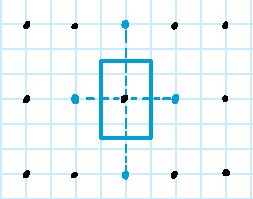
\includegraphics[width=0.4\linewidth]{resources/09-05-2012/BZ1.pdf}
        \caption[1. BZ Rechteckgitter]{1. Brillouin-Zone eines Rechteckgitters}
        \label{fig:BZ1_rechteckgitter}
    \end{samepage}
\end{figure}
\begin{enumerate}
    \item Reziprokes Gitter aufzeichen
    \item Zellenmittelpunkt wählen
    \item Vom Mittelpunkt in beide Dimensionen den nächstgelegenen Gitterpunkt finden
    \item Mittelpunkt mit diesen Punkten verbinden
    \item Auf den Mittelpunkt der Verbindenden eine Orthogonale zeichnen
\end{enumerate}

\question{Wodurch unterscheiden sich akustische von optischen Phononen?}
\label{q:29}

Ein Phonon ist die elementare Anregung (Quant) des elastischen Feldes. Sie beschreiben die elementare bzw. kollektive Anregungen der Gitterschwingungen eines Festkörpers.
In einem dreidimensionalen Kristall mit $N$ Atomen in der primitiven Basis existieren zu jedem mit der Kristallsymmetrie verträglichen Wellenvektor 
$3N$ mögliche Schwingungsmoden:

\begin{itemize}
    \item Akustische Phononen: Diese Phononen werden auch als Schallquanten bezeichnet und sind die Quanten der Schallwellen, die sich durch das Kristallgitter fortpflanzen.
          Alle Quanten bewegen sich hier in einer Einheitszelle in Phase und haben 3 akustische Moden, wovon eine longitudinal und zwei transversal sind.

          \begin{figure}[H]
            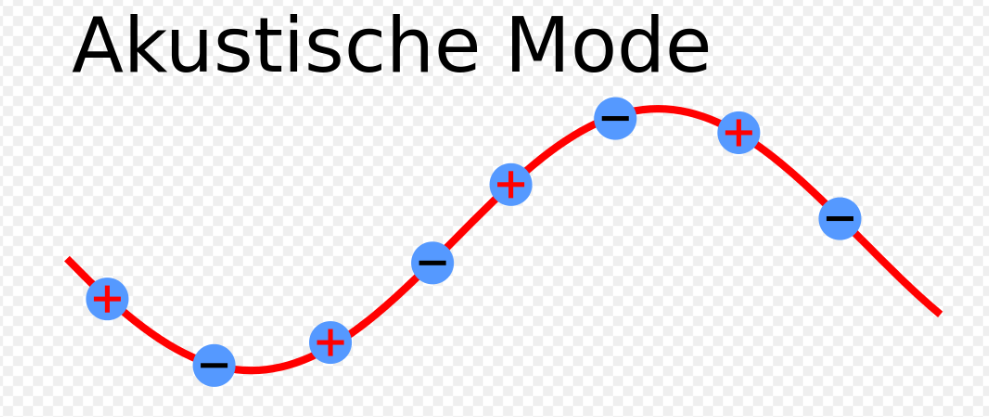
\includegraphics[width=0.8\linewidth]{resources/09-05-2012/akust.PNG}
            \caption{Darstellung von akustischen Transversalwellen von Phononen}
          \end{figure}
    \item Optische Phononen: Diese Phononen bewegen sich in einer Basisgegenphasig, wodurch es Schwingungsmodi gibt, bei denen entgegengesetzt geladene Untergitter gegeneinander schwingen. 
          Die dabei oszillierenden Dipolmomente können mit Photonen wechselwirken. Oft kommen solche Kopplungen im Infrarotbereich, also der Wärmebewegung in Festkörpern vor.
          Beispiele für solche infrarot-aktiven Gitter sind Ionengitter wie Natriumchloridkristalle.

          \begin{figure}[H]
            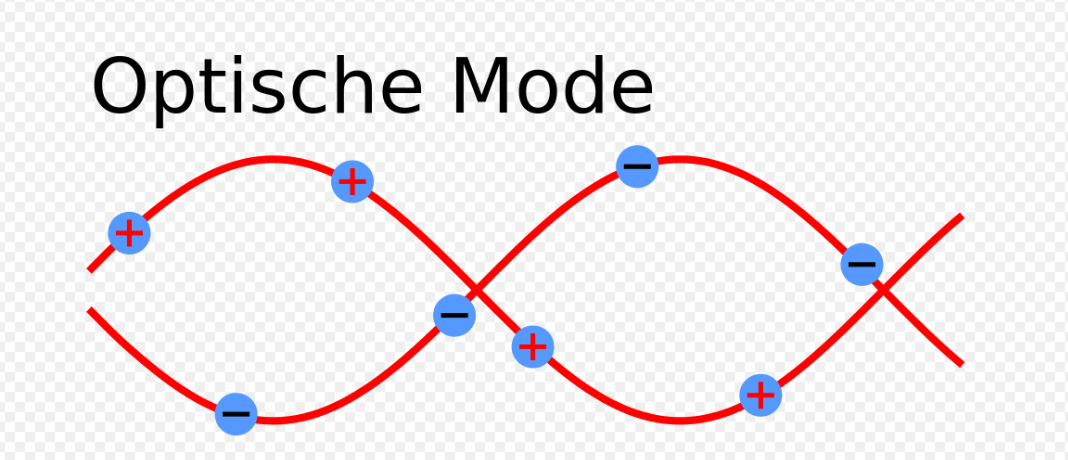
\includegraphics[width=0.8\linewidth]{resources/09-05-2012/opt.PNG}
            \caption{Darstellung von optischen Phononen}
          \end{figure}
\end{itemize}



\question{Vergleiche die Einstein- und Debye-Modelle der spez. Wärme. Welche Annahme ist im 
Einstein Modell zu einfach?}
\label{q:30}

\begin{figure}[H]  
    \centering
    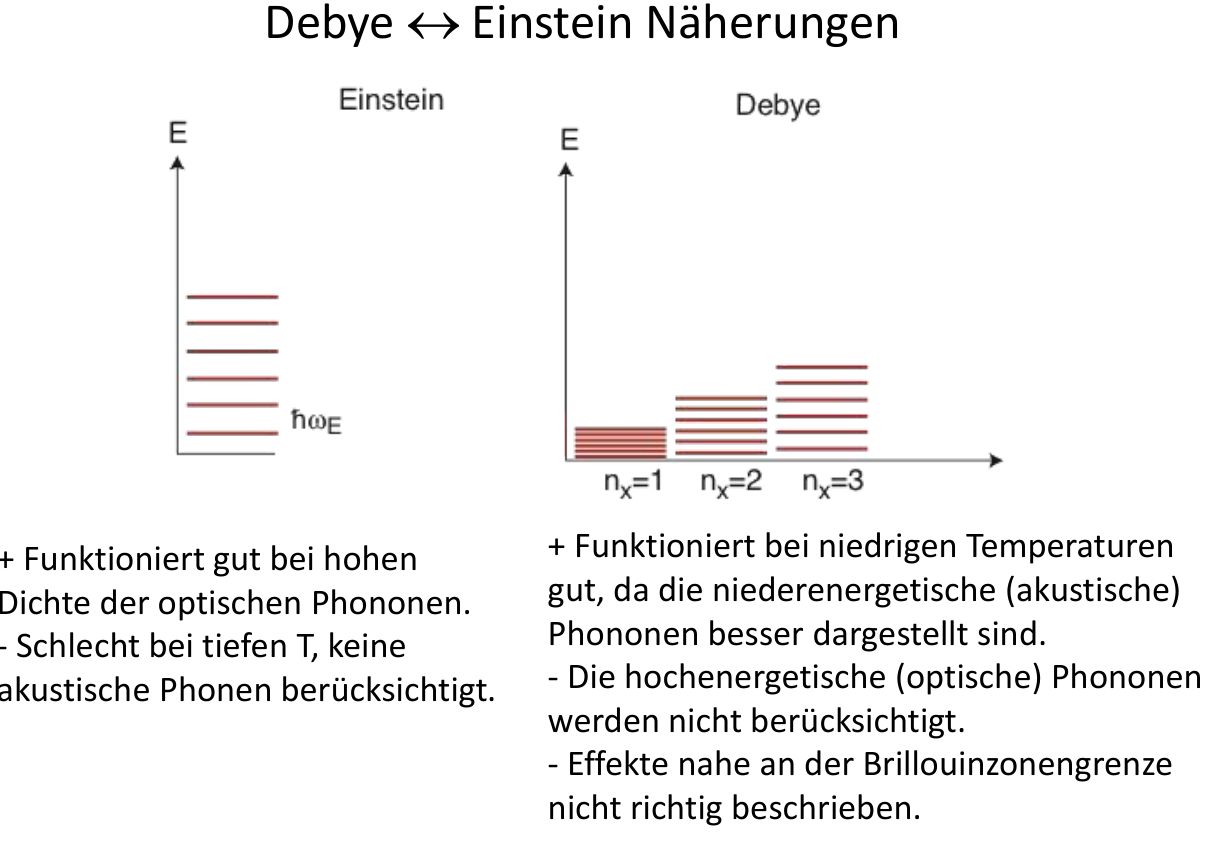
\includegraphics[width=.8\textwidth]{resources/09-05-2012/q30.png}
    \caption{Vergleich zwischen Einstein- und Debye-Modell.}
\end{figure}

Das Einsteinmodell nimmt an, dass alle Atome im Kristall mit der gleichen Frequenz schwingen, zudem werden keine akustischen Phononen berücksichtigt.

\newpage
